\documentclass{beamer}
\graphicspath{ {graphics/} }
\begin{document}
\title{Literary Worlds Javascript Client}   
\author{John Lewis, Owen Watson, Tim Cunningham} 
\date{\today} 
\usenavigationsymbolstemplate{}
\frame{\titlepage}

\frame{\frametitle{Overview} 
Literary Worlds is an multiuser text based game used for English education at WMU.\\
Most of these text based games provide a telnet interface for playing, Literary Worlds uses MOOTcan, a Java applet.\\
The aim of this project is to provide a drop-in replacement user interface in Javascript.\\
}

\frame{
\begin{centering}
\centering

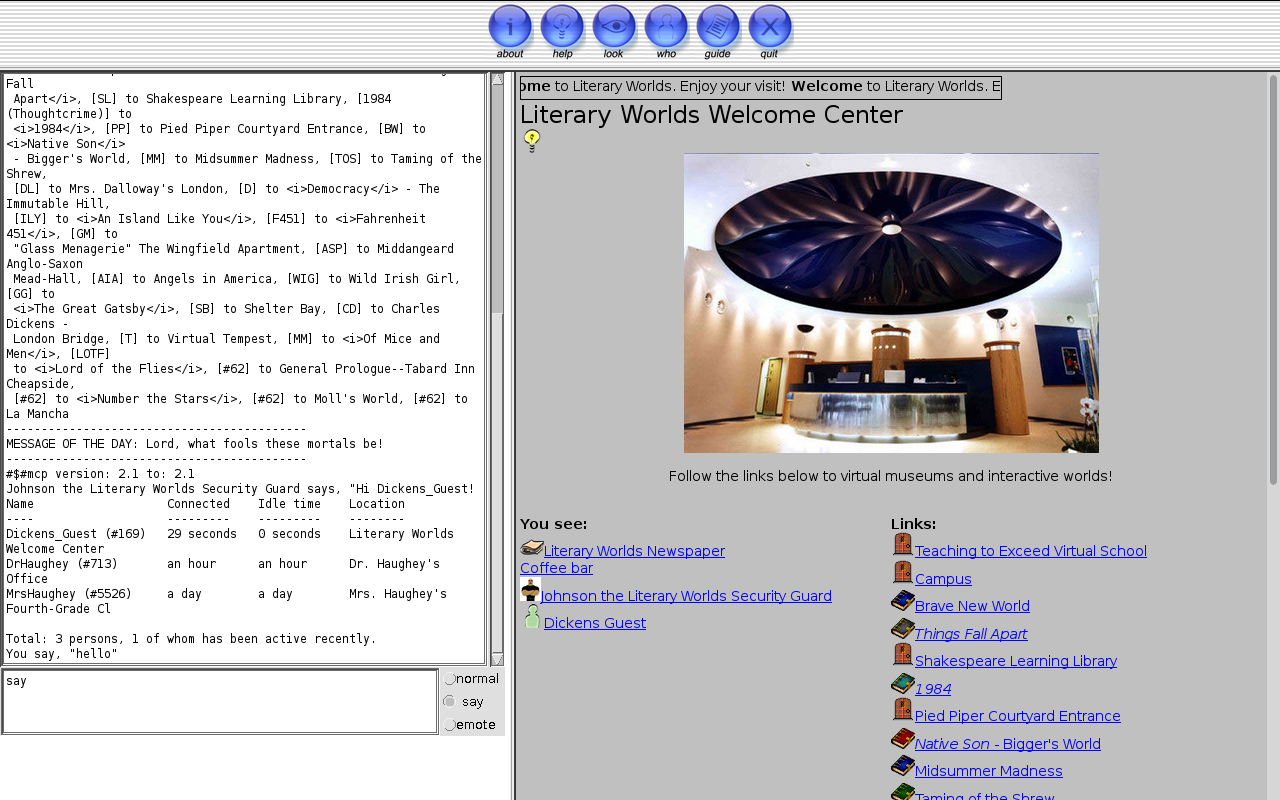
\includegraphics[width=\textwidth,height=\textheight,keepaspectratio]{classUsage.png}
\end{centering}
}

\end{document}
